%%%%%%%%%%%%%%%%%%%%%%%%%%%%%%%%%%%%%%%%%
% Beamer Presentation
% LaTeX Template
% Version 1.0 (10/11/12)
%
% This template has been downloaded from:
% http://www.LaTeXTemplates.com
%
% License:
% CC BY-NC-SA 3.0 (http://creativecommons.org/licenses/by-nc-sa/3.0/)
%
%%%%%%%%%%%%%%%%%%%%%%%%%%%%%%%%%%%%%%%%%

%----------------------------------------------------------------------------------------
%	PACKAGES AND THEMES
%----------------------------------------------------------------------------------------

\documentclass{beamer}

\mode<presentation>{% The Beamer class comes with a number of default slide themes
% which change the colors and layouts of slides. Below this is a list
% of all the themes, uncomment each in turn to see what they look like.

%\usetheme{default}
%\usetheme{AnnArbor}
%\usetheme{Antibes}
%\usetheme{Bergen}
%\usetheme{Berkeley}
\usetheme[compress]{Berlin}
%\usetheme{Boadilla}
%\usetheme{CambridgeUS}
%\usetheme{Copenhagen}
%\usetheme{Darmstadt}
%\usetheme{Dresden}
%\usetheme{Frankfurt}
%\usetheme{Goettingen}
%\usetheme{Hannover}
%\usetheme{Ilmenau}
%\usetheme{JuanLesPins}
%\usetheme{Luebeck}
%\usetheme{Madrid}
%\usetheme{Malmoe}
%\usetheme{Marburg}
%\usetheme{Montpellier}
%\usetheme{PaloAlto}
%\usetheme{Pittsburgh}
%\usetheme{Rochester}
%\usetheme{Singapore}
%\usetheme{Szeged}
%\usetheme{Warsaw}

% As well as themes, the Beamer class has a number of color themes
% for any slide theme. Uncomment each of these in turn to see how it
% changes the colors of your current slide theme.

%\usecolortheme{albatross}
%\usecolortheme{beaver}
%\usecolortheme{beetle}
%\usecolortheme{crane}
%\usecolortheme{dolphin}
%\usecolortheme{dove}
%\usecolortheme{fly}
%\usecolortheme{lily}
%\usecolortheme{orchid}
%\usecolortheme{rose}
%\usecolortheme{seagull}
%\usecolortheme{seahorse}
%\usecolortheme{whale}
%\usecolortheme{wolverine}

\makeatother
\setbeamertemplate{footline}
{
  \leavevmode%
  \hbox{%
  \begin{beamercolorbox}[wd=.3\paperwidth,ht=2.25ex,dp=1ex,center]{section in head/foot}%
    \usebeamerfont{author in head/foot}\insertshortauthor
  \end{beamercolorbox}%
  \begin{beamercolorbox}[wd=.6\paperwidth,ht=2.25ex,dp=1ex,center]{subsection in head/foot}%
    \usebeamerfont{title in head/foot}\insertshorttitle
  \end{beamercolorbox}%
  \begin{beamercolorbox}[wd=.1\paperwidth,ht=2.25ex,dp=1ex,center]{title}%
    \usebeamerfont{instritute in head/foot}\insertshortinstitute
  \end{beamercolorbox}}%
  \vskip0pt%
}
\makeatletter

%\setbeamertemplate{footline} % To remove the footer line in all slides uncomment this line
%\setbeamertemplate{footline}[page number] % To replace the footer line in all slides with a simple slide count uncomment this line

\setbeamertemplate{navigation symbols}{} % To remove the navigation symbols from the bottom of all slides uncomment this line
}

\usepackage[english]{babel} 
\usepackage[utf8x]{inputenc}

\usepackage{graphicx} % Allows including images
\usepackage{booktabs} % Allows the use of \toprule, \midrule and \bottomrule in tables
\usepackage{multicol} 

% Math packages
\usepackage{amsmath}
\usepackage{mathtools}
\usepackage{amssymb}
\usepackage{mathpartir}

%----------------------------------------------------------------------------------------
%	TITLE PAGE
%----------------------------------------------------------------------------------------

\title[Mathematical Foundations and the Foundational Crisis]{Foundations of Mathematics\\and the Foundational Crisis} % The short title appears at the bottom of every slide, the full title is only on the title page

\author{Kevin Kappelmann} % Your name
\institute[TUM] % Your institution as it will appear on the bottom of every slide, may be shorthand to save space
{Technical University of Munich}
\date{\today} % Date, can be changed to a custom date

\begin{document}

\begin{frame}
\titlepage % Print the title page as the first slide
\end{frame}

%----------------------------------------------------------------------------------------
%	PRESENTATION SLIDES
%----------------------------------------------------------------------------------------
\section*{Introduction}
%------------------------------------------------

\begin{frame}
    \frametitle{}
    \begin{itemize}[<+->]
	\item What is the most exact science of humanity?
	\begin{itemize}
		\item Well, obviously it is maths, right?
	\end{itemize}
	\item I shall convince you with rigorous proofs!
	\begin{itemize}
		\item What is a proof?
		\item What is logical?
	\end{itemize}
	\item Can we trust each other?
	\item Can we trust a computer?
    \end{itemize}
\end{frame}

\begin{frame}
    \frametitle{}
    \begin{itemize}[<+->]
	\item When do I accept a proof?
	\begin{itemize}
		\item Do I need to understand every isolated step?
		\item Do I need to understand its holistic idea?
	\end{itemize}
	\item Computer-generated proofs are barely verifiable by hand.
	\begin{itemize}
		\item[$\Rightarrow$] Controversies
	\end{itemize}
	\item But it is not the first controversy in mathematical history\ldots
    \end{itemize}
\end{frame}


%------------------------------------------------
% Overview slide
%------------------------------------------------

\begin{frame}
    \frametitle{Overview} 
    %\begin{multicols}{2}
        \tableofcontents
    %\end{multicols}
\end{frame}

%------------------------------------------------
\section{History of Mathematics}
%------------------------------------------------
\subsection{First steps}
\begin{frame}
    \frametitle{1+1=2}
    \begin{itemize}[<+->]
	\item How did it begin?
	\begin{itemize}
		\item One apple and another apple are two apples.
		\item One banana and another banana are two bananas.
		\item[$\Rightarrow$] One and one is two!
	\end{itemize}
	\item Maths is about abstraction.
	\item Numbers were the first abstraction.
    \end{itemize}
\end{frame}
\begin{frame}
    \frametitle{Intuitive Work}
    \begin{itemize}[<+->]
	\item What also seems quite intuitive?
	\begin{itemize}
		\item Drawing shapes
	\end{itemize}
	\item Arithmetic and geometry were the first branches of mathematics.
	\item First complex mathematics around 2400 BC in Egypt and Babylonia
	\item Maths served as an applied tool.
	\begin{itemize}
		\item No proofs, but heuristics and pictures
	\end{itemize}
    \end{itemize}
\end{frame}
\subsection{Ancient Greece}
\begin{frame}
    \frametitle{Q.E.D.}
    \begin{itemize}[<+->]
	\item Ancient Greeks developed the notion of a proof in 600 BC.
	\item The Pythagoreans discovered irrational numbers.
	\begin{itemize}
		\item[$\Rightarrow$] First controversy of mathematics
	\end{itemize}
	\item Euclid's Elements around 300 BC
	\begin{itemize}
		\item Axiomatic, deductive treatment of mathematics similar to modern systems
		\item A work of timeless certainty\ldots\\\uncover<+->{\ldots at least so had been thought}
	\end{itemize}
	%\item Zeno of Elea devised four paradoxes.
    \end{itemize}
\end{frame}
%\begin{frame}
    %\frametitle{Come on, Achilles!}
    %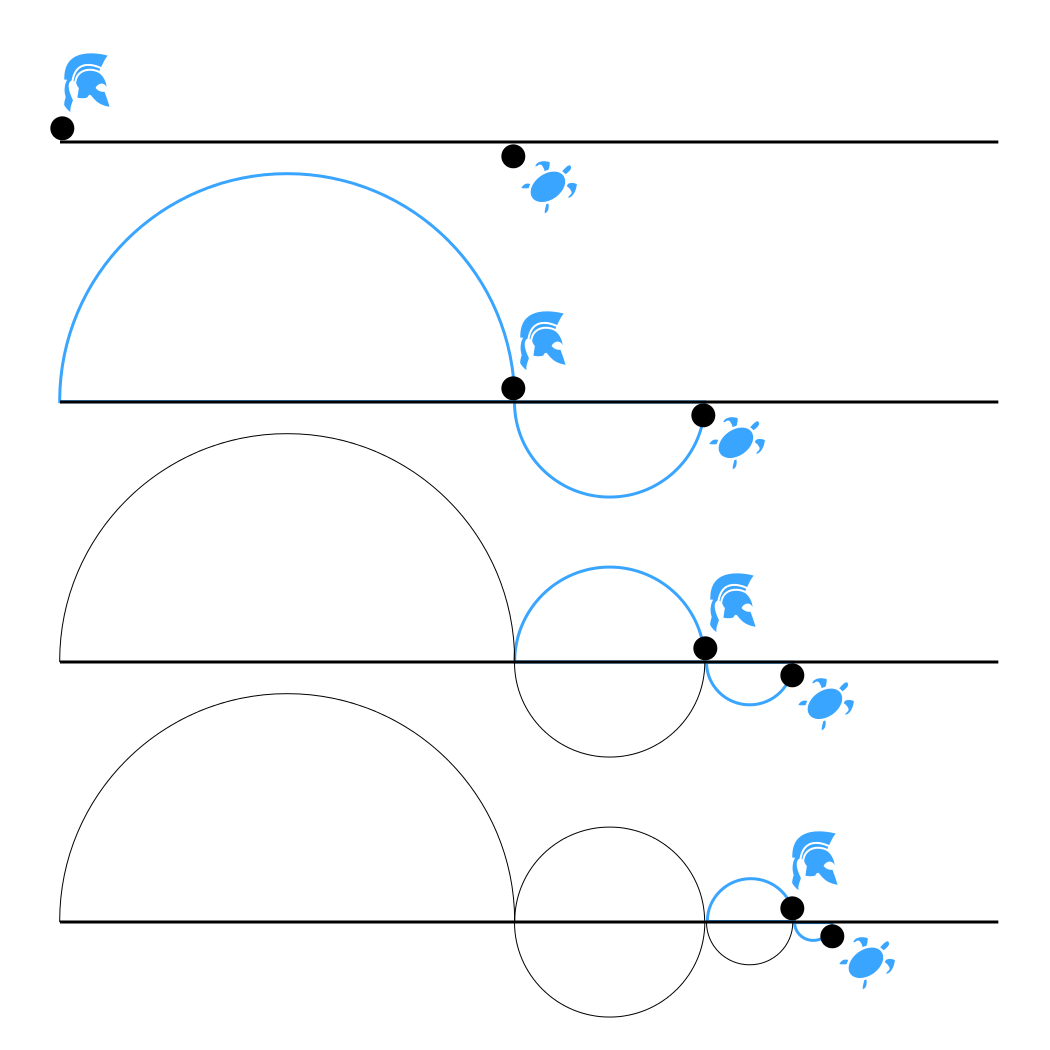
\includegraphics[height=0.6\paperheight]{achilles_tortoise.png}
    %\begin{itemize}[<+->]
	%\item Ancient Greeks developed notion of proof in 600 BC.
	%\item Pythagoreans discovered irrational numbers.
	%\begin{itemize}
		%\item[$\Rightarrow$] First controversy of mathematics
	%\end{itemize}
	%\item Zeno of Elea devised four paradoxes.
    %\end{itemize}
%\end{frame}
\begin{frame}
    \frametitle{Euclid's Postulates}
	``Let the following be postulated:\pause
     \begin{enumerate}[<+->]
	\item To draw a straight line from any point to any point.
	\item To produce [extend] a finite straight line continuously in a straight line.
	\item To describe a circle with any centre and distance [radius].
	\item That all right angles are equal to one another.
	\item That, if a straight line falling on two straight lines make the interior angles on the same side less than two right angles, the two straight lines, if produced indefinitely, meet on that side on which are the angles less than the two right angles.''
     \end{enumerate}
\end{frame}
%------------------------------------------------
\section{Foundational Crisis}
%------------------------------------------------
\subsection{Causes}
\begin{frame}
    \frametitle{Search for foundations}
    \begin{itemize}[<+->]
	\item Gauß proved the independence of Euclid's fifth postulate in 1813.
	\begin{itemize}
		\item[$\Rightarrow$] Scepticism towards used systems
	\end{itemize}
	\item Rigorous axiomatisation of mathematical branches in the late 19th century
	\begin{itemize}
		\item Arithmetic of natural numbers by Peano
		\item Geometry by Hilbert and Pasch
		\item Predicate logic by Frege
	\end{itemize}
	\item Desire for universal and consistent system
    \end{itemize}
\end{frame}
\begin{frame}
    \frametitle{Cantor's realm}
    \begin{itemize}[<+->]
	\item \textit{``A set is a gathering together into a whole of definite, distinct objects of our perception or of our thought --- which are called elements of the set.''}\cite{cantor_set} --- Georg Cantor
	\item Certainly universal\ldots\\\uncover<+->{\ldots but informal and thus not adequate for a study of consistency}
	\item Frege tried to build a mathematical foundation with logic.
    \end{itemize}
\end{frame}
\begin{frame}
    \frametitle{Here comes the Russell}
    \begin{itemize}[<+->]
	\item Frege tried to build a mathematical foundation with logic.
    \end{itemize}
\end{frame}
%------------------------------------------------
\subsection{Logicism}
\begin{frame}
    \frametitle{}
\end{frame}
%------------------------------------------------
\subsection{Formalism}
\begin{frame}
    \frametitle{}
\end{frame}
%------------------------------------------------
\subsection{Intuitionism}
\begin{frame}
    \frametitle{}
\end{frame}
%------------------------------------------------
\subsection{Peak and End}
\begin{frame}
    \frametitle{}
\end{frame}
%------------------------------------------------
\section{Aftermath and Prospects}
\begin{frame}
    \frametitle{}
\end{frame}
%------------------------------------------------
\section*{}
%------------------------------------------------
\begin{frame}
    \Huge{\centerline{The End}}
\end{frame}
%----------------------------------------------------------------------------------------

\newpage
\bibliographystyle{plain}
\bibliography{../../paper/sources.bib}
\end{document} 
